\chapter{Binary Numbers, Bits and Boolean Algebra}
\label{ch:binary}

We now have switches (transistors). Before wiring them into logic, we need the language that logic speaks: binary numbers and Boolean algebra. This chapter covers how computers represent numbers, how to manipulate individual bits (a favorite topic of the coding part of the assessment), and the algebra used to design and simplify logic circuits.

\section{Why two values?}

A wire's voltage can take any value, so why do computers use only two, 0 and 1? Because of \emph{noise}. Every real signal picks up small unwanted disturbances: from neighboring wires, from the power supply, from temperature. If we tried to represent ten different values with ten voltage levels between 0 and 1\,V, levels would be only 0.1\,V apart, and a little noise would turn a 6 into a 7.

With only two values, we can treat \emph{any} voltage near 0 as a 0 and \emph{any} voltage near the supply as a 1, with a wide forbidden zone between. Noise has to be enormous to flip a value. Better still, each logic gate restores its output to a clean 0 or 1, so noise does not accumulate as signals pass through many gates (Chapter~\ref{ch:cmos}). Two values are the most robust choice.

One binary digit is a \term{bit}. Groups of bits have names: 4 bits are a \term{nibble}, 8 bits a \term{byte}, and a \term{word} is the natural size a processor works with (often 32 or 64 bits).

\section{Binary numbers}

In decimal, each digit position is worth ten times the one to its right: $347 = 3\times100 + 4\times10 + 7\times1$. In binary, each position is worth \emph{two} times the one to its right:
\[
  1011_2 = 1\times8 + 0\times4 + 1\times2 + 1\times1 = 11_{10}.
\]
The rightmost bit is the \term{least significant bit} (LSB); the leftmost is the \term{most significant bit} (MSB).

\paragraph{Decimal to binary.} Repeatedly divide by 2 and record the remainders; read them from last to first. For 45: $45/2 = 22$ r1, $22/2 = 11$ r0, $11/2 = 5$ r1, $5/2 = 2$ r1, $2/2 = 1$ r0, $1/2 = 0$ r1. Reading upward: $45 = 101101_2$. Check: $32+8+4+1 = 45$.

\paragraph{Powers of two to know by heart.}
\begin{center}
\begin{tabular}{ccccccc}
\toprule
$2^0$ & $2^1$ & $2^2$ & $2^3$ & $2^4$ & $2^5$ & $2^6$ \\
1 & 2 & 4 & 8 & 16 & 32 & 64 \\
\midrule
$2^7$ & $2^8$ & $2^{10}$ & $2^{12}$ & $2^{16}$ & $2^{20}$ & $2^{32}$ \\
128 & 256 & 1024 & 4096 & 65\,536 & 1\,048\,576 & $\approx 4.3\times10^9$ \\
\bottomrule
\end{tabular}
\end{center}

In computing, a ``kilobyte'' of memory usually means $2^{10} = 1024$ bytes (strictly a kibibyte, KiB), a ``megabyte'' $2^{20}$ bytes, and a ``4\,KB page'' is $2^{12} = 4096$ bytes.

\section{Hexadecimal}

Long binary strings are hard to read, so engineers write them in \term{hexadecimal} (base 16). Each hex digit stands for exactly 4 bits, using 0--9 then A--F for 10--15:

\begin{center}
\begin{tabular}{cccccccc}
\toprule
0 & 1 & 2 & 3 & 4 & 5 & 6 & 7 \\
0000 & 0001 & 0010 & 0011 & 0100 & 0101 & 0110 & 0111 \\
\midrule
8 & 9 & A & B & C & D & E & F \\
1000 & 1001 & 1010 & 1011 & 1100 & 1101 & 1110 & 1111 \\
\bottomrule
\end{tabular}
\end{center}

To convert binary to hex, split into groups of four from the right: $1011\,0111_2 = \text{B7}_{16}$. In code, hex is written with a \code{0x} prefix: \code{0xB7} $= 11\times16 + 7 = 183$. Memory addresses are almost always written in hex.

\section{How many values fit in $n$ bits?}

Each bit doubles the number of possible patterns, so $n$ bits can represent $2^n$ different values. Going the other way, to represent $N$ different things you need
\[
  n = \lceil \log_2 N \rceil \text{ bits}
\]
(the ceiling $\lceil\cdot\rceil$ means round up). For 1000 values: $2^9 = 512$ is too few, $2^{10} = 1024$ is enough, so 10 bits. This calculation appears constantly: how many flip-flops a state machine needs (Chapter~\ref{ch:fsm}), how many address bits a memory needs, how many select lines a multiplexer needs.

\section{Negative numbers: two's complement}
\label{sec:twos}

Computers almost always store signed integers in \term{two's complement}. The idea is simple: the MSB gets a \emph{negative} weight. For 8 bits, the place values are
\[
  -128,\; 64,\; 32,\; 16,\; 8,\; 4,\; 2,\; 1.
\]
So $1111\,1111_2 = -128 + 127 = -1$, and $1000\,0000_2 = -128$.

\begin{itemize}
  \item Range of $n$-bit two's complement: $-2^{n-1}$ to $2^{n-1}-1$. For 8 bits: $-128$ to $127$.
  \item The MSB tells the sign: 1 means negative.
  \item \textbf{To negate a number: invert every bit, then add 1.}
\end{itemize}

\begin{worked}{representing $-20$ in 8 bits}
$+20 = 0001\,0100$. Invert: $1110\,1011$. Add 1: $1110\,1100$. Check with weights: $-128 + 64 + 32 + 8 + 4 = -20$. Correct.
\end{worked}

The beauty of two's complement is that ordinary binary addition works for signed numbers too: the same adder hardware handles both, and subtraction is just adding the negation, $A - B = A + \nt{B} + 1$ (Chapter~\ref{ch:comb}).

\paragraph{Overflow.} If a result does not fit in $n$ bits, it wraps around. In 8 bits, $127 + 1$ gives $1000\,0000 = -128$. Signed overflow happens exactly when two numbers of the same sign are added and the result has the opposite sign.

\paragraph{Sign extension.} To widen a two's complement number, copy its sign bit into the new upper bits: $-3$ in 4 bits is $1101$; in 8 bits it is $1111\,1101$.

\section{Bitwise operations}
\label{sec:bitops}

Programming languages (and hardware) can operate on every bit of a word at once:

\begin{center}
\begin{tabular}{llll}
\toprule
Operation & C syntax & Rule per bit & Example (\code{1100} op \code{1010}) \\
\midrule
AND & \code{a \& b} & 1 only if both are 1 & \code{1000} \\
OR & \code{a | b} & 1 if either is 1 & \code{1110} \\
XOR & \code{a \^{} b} & 1 if they differ & \code{0110} \\
NOT & \code{\~{}a} & flip every bit & \code{\~{}1100 = 0011} \\
Left shift & \code{a << k} & move bits left, fill with 0 & \code{0011 << 1 = 0110} \\
Right shift & \code{a >> k} & move bits right & \code{1100 >> 2 = 0011} \\
\bottomrule
\end{tabular}
\end{center}

Shifting left by $k$ multiplies by $2^k$; shifting right by $k$ divides by $2^k$ (rounding down) for unsigned numbers. So with \code{i = 8} and \code{j = 2}, \code{i << j} is 32 and \code{i >> j} is 2. For \emph{signed} numbers, a right shift usually copies the sign bit in from the left (an \term{arithmetic shift}) so negative numbers stay negative; unsigned values get zeros (a \term{logical shift}).

\subsection*{Bit tricks worth knowing}

Using a \term{mask} (a word with 1s only where you care), you can work on individual bits:

\begin{center}
\begin{tabular}{ll}
\toprule
Goal & Expression \\
\midrule
Read bit $k$ & \code{(x >> k) \& 1} \\
Set bit $k$ to 1 & \code{x | (1 << k)} \\
Clear bit $k$ to 0 & \code{x \& \~{}(1 << k)} \\
Toggle bit $k$ & \code{x \^{} (1 << k)} \\
Keep only the lowest set bit & \code{x \& (-x)} \\
Clear the lowest set bit & \code{x \& (x - 1)} \\
Is $x$ a power of two? & \code{x != 0 \&\& (x \& (x - 1)) == 0} \\
Mask of bits \code{lo} to \code{hi} & \code{((1 << (hi - lo + 1)) - 1) << lo} \\
\bottomrule
\end{tabular}
\end{center}

Why does \code{x \& (x-1)} clear the lowest set bit? Subtracting 1 flips the lowest 1 to 0 and all the 0s below it to 1s, and leaves everything above unchanged. ANDing with the original keeps the upper bits and zeros the rest. A power of two has exactly one 1 bit, so clearing it leaves zero.

\begin{worked}{building a bit mask}
Build a mask with 1s in bits 4 through 7. Width $= 7 - 4 + 1 = 4$. \code{(1 << 4) - 1} $= 1111_2$. Shift left by 4: $1111\,0000_2 =$ \code{0xF0}. (Careful: if the width is the full 32 bits, \code{1 << 32} overflows a 32-bit integer in C; use a 64-bit type for the intermediate value.)
\end{worked}

\begin{worked}{are two addresses on the same 4\,KB page?}
Memory is divided into pages of $4096 = 2^{12}$ bytes. The low 12 bits of an address are the offset within a page; the remaining upper bits are the \emph{page number}. Two addresses are on the same page exactly when their page numbers match:
\begin{center}
\code{(a >> 12) == (b >> 12)} \qquad or equivalently \qquad \code{((a \^{} b) \& \~{}0xFFF) == 0}
\end{center}
\code{0x12345FF0} and \code{0x12345010}: both have page number \code{0x12345}, so same page. \code{0x12345FFF} and \code{0x12346000}: page numbers \code{0x12345} and \code{0x12346}, so different pages, even though the addresses differ by only 1.
\end{worked}

\begin{onoa}
Both of the worked examples above match coding problems reported on NVIDIA's Ignite assessment: building a bit mask from bit \code{lo} to bit \code{hi}, and checking whether two 32-bit addresses fall on the same 4\,KB page. Chapter~\ref{ch:prog} has full code.
\end{onoa}

\subsection*{XOR, the most useful operator}

XOR has algebraic properties that make it a favorite in puzzles and in hardware:
\begin{itemize}
  \item $a \oplus 0 = a$ and $a \oplus a = 0$: XORing with a value twice cancels it.
  \item $a \oplus 1 = \nt{a}$: XOR with 1 inverts. So XOR is a \emph{controlled inverter}.
  \item XOR is commutative and associative, so order does not matter.
  \item The XOR of all bits of a word is its \term{parity}: 1 if it has an odd number of 1s.
\end{itemize}
A consequence used in coding problems: if $P_i$ is the XOR of the first $i$ elements of an array (a \term{prefix XOR}), then the XOR of elements $l$ through $r$ is $P_{r+1} \oplus P_l$, because everything before $l$ appears twice and cancels.

\section{Gray code}
\label{sec:gray}

In ordinary binary, counting from 3 ($011$) to 4 ($100$) changes three bits at once. If those bits are read at the wrong moment, while some have changed and some have not, you can get any value at all. \term{Gray code} orders the numbers so that \emph{exactly one bit changes} between neighbors:

\begin{center}
\begin{tabular}{lcccccccc}
\toprule
Decimal & 0 & 1 & 2 & 3 & 4 & 5 & 6 & 7 \\
Binary & 000 & 001 & 010 & 011 & 100 & 101 & 110 & 111 \\
Gray & 000 & 001 & 011 & 010 & 110 & 111 & 101 & 100 \\
\bottomrule
\end{tabular}
\end{center}

Conversion: $g = b \oplus (b \gg 1)$. Gray code is used for counters that are read by a different clock (Chapter~\ref{ch:rtl}) and to label Karnaugh maps (below).

\section{Boolean algebra}

\term{Boolean algebra}, named after George Boole, is the mathematics of variables that are only 0 or 1. It has three basic operations:
\begin{itemize}
  \item AND, written $A \cdot B$ or just $AB$: 1 only if both are 1.
  \item OR, written $A + B$: 1 if at least one is 1. (Here $1 + 1 = 1$.)
  \item NOT, written $\nt{A}$ (or $A'$): the opposite value.
\end{itemize}
Precedence, as in ordinary algebra: NOT first, then AND, then OR. So $A + BC$ means $A + (B \cdot C)$.

Combined truth table of the common two-input functions:
\begin{center}
\begin{tabular}{cc|ccccccc}
\toprule
$A$ & $B$ & AND & OR & NAND & NOR & XOR & XNOR \\
\midrule
0 & 0 & 0 & 0 & 1 & 1 & 0 & 1 \\
0 & 1 & 0 & 1 & 1 & 0 & 1 & 0 \\
1 & 0 & 0 & 1 & 1 & 0 & 1 & 0 \\
1 & 1 & 1 & 1 & 0 & 0 & 0 & 1 \\
\bottomrule
\end{tabular}
\end{center}

\subsection*{The laws}

\begin{center}
\begin{tabular}{lll}
\toprule
Law & OR form & AND form \\
\midrule
Identity & $A + 0 = A$ & $A \cdot 1 = A$ \\
Null & $A + 1 = 1$ & $A \cdot 0 = 0$ \\
Idempotent & $A + A = A$ & $A \cdot A = A$ \\
Complement & $A + \nt{A} = 1$ & $A \cdot \nt{A} = 0$ \\
Involution & \multicolumn{2}{l}{$\nt{\nt{A}} = A$} \\
Commutative & $A + B = B + A$ & $AB = BA$ \\
Associative & $(A+B)+C = A+(B+C)$ & $(AB)C = A(BC)$ \\
Distributive & $A + BC = (A+B)(A+C)$ & $A(B+C) = AB + AC$ \\
Absorption & $A + AB = A$ & $A(A+B) = A$ \\
Also useful & $A + \nt{A}B = A + B$ & $A(\nt{A} + B) = AB$ \\
De Morgan & $\nt{A + B} = \nt{A}\,\nt{B}$ & $\nt{AB} = \nt{A} + \nt{B}$ \\
Consensus & \multicolumn{2}{l}{$AB + \nt{A}C + BC = AB + \nt{A}C$} \\
\bottomrule
\end{tabular}
\end{center}

Two of these surprise people because they do not hold in ordinary algebra: $A + 1 = 1$, and the first distributive law $A + BC = (A+B)(A+C)$. Check any law yourself with a truth table; that is always a valid proof.

\begin{bigidea}
\textbf{De Morgan's laws}: to complement an expression, swap AND with OR and complement each variable. ``Not (A or B)'' is ``not A and not B.'' These laws are why a NAND gate is the same as an OR gate with inverted inputs, and they are the key to building logic from transistors (Chapter~\ref{ch:cmos}).
\end{bigidea}

\begin{worked}{simplifying}
Simplify $F = AB + A\nt{B} + \nt{A}B$.

$AB + A\nt{B} = A(B + \nt{B}) = A$. So $F = A + \nt{A}B = A + B$.
\end{worked}

\section{From a truth table to an expression}

Any truth table can be turned into a formula:

\begin{itemize}
  \item \textbf{Sum of products (SOP)}: for each row where the output is 1, write an AND term (a \term{minterm}) that is 1 only for that row, then OR them all. For $A=0, B=1$, the minterm is $\nt{A}B$.
  \item \textbf{Product of sums (POS)}: for each row where the output is 0, write an OR term (a \term{maxterm}) that is 0 only for that row, then AND them.
\end{itemize}

Minterms are numbered by the row's binary value; $F = \sum m(1,2)$ means ``1 in rows 1 and 2.'' For two inputs, that is $\nt{A}B + A\nt{B} = A \oplus B$.

\paragraph{How many functions are there?} An $n$-input truth table has $2^n$ rows, and each row's output can be 0 or 1 independently, so there are $2^{2^n}$ different functions. For 2 inputs: $2^4 = 16$. For 3 inputs: $2^8 = 256$.

\section{Karnaugh maps}

A \term{Karnaugh map} (K-map) is a truth table drawn as a grid so that simplifications become visible. Rows and columns are labeled in Gray code, so any two neighboring cells differ in exactly one variable. When two neighboring cells are both 1, that variable does not matter, and the two minterms merge into one simpler term.

Rules for grouping the 1s:
\begin{enumerate}
  \item Groups are rectangles of 1, 2, 4, 8 or 16 cells (powers of two).
  \item Groups may wrap around the edges: the left column neighbors the right column, and the top row neighbors the bottom row (the four corners are neighbors too).
  \item Make each group as large as possible, and use as few groups as possible. Groups may overlap.
  \item Each group becomes one product term containing only the variables that stay constant across the group.
  \item ``Don't care'' cells (inputs that never occur, written $X$) may be included in groups if that helps, or ignored.
\end{enumerate}

\begin{figure}[h]
\centering
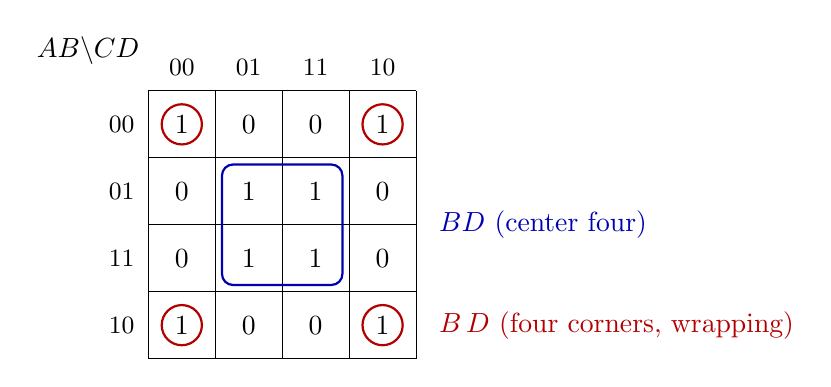
\begin{tikzpicture}[scale=0.85]
  \foreach \i in {0,...,4} { \draw (\i,0) -- (\i,4); \draw (0,\i) -- (4,\i); }
  \node at (-0.9,4.6) {$AB \backslash CD$};
  \foreach \lab [count=\c from 0] in {00,01,11,10} {
    \node at (\c+0.5,4.35) {\small \lab};
    \node at (-0.4,3.5-\c) {\small \lab};}
  % rows: 00: 1 0 0 1 ; 01: 0 1 1 0 ; 11: 0 1 1 0 ; 10: 1 0 0 1
  \foreach \c/\r/\v in {0/0/1,1/0/0,2/0/0,3/0/1, 0/1/0,1/1/1,2/1/1,3/1/0,
                       0/2/0,1/2/1,2/2/1,3/2/0, 0/3/1,1/3/0,2/3/0,3/3/1}
    \node at (\c+0.5,3.5-\r) {\v};
  \draw[blue!70!black,thick,rounded corners] (1.1,1.1) rectangle (2.9,2.9);
  \node[blue!70!black,right] at (4.2,2) {$BD$ (center four)};
  \foreach \c/\r in {0/0,3/0,0/3,3/3}
    \draw[red!70!black,thick] (\c+0.5,3.5-\r) circle (0.3);
  \node[red!70!black,right] at (4.2,0.5) {$\nt{B}\,\nt{D}$ (four corners, wrapping)};
\end{tikzpicture}
\caption{K-map for $F = \sum m(0,2,5,7,8,10,13,15)$. Two groups of four give $F = BD + \nt{B}\,\nt{D}$.}
\label{fig:kmap}
\end{figure}

\begin{worked}{a four-variable K-map}
Simplify $F(A,B,C,D) = \sum m(0,2,5,7,8,10,13,15)$ (Figure~\ref{fig:kmap}).

The center four cells have $B=1$ and $D=1$ while $A$ and $C$ vary: the group is $BD$. The four corner cells are neighbors through wrap-around; they have $B = 0$ and $D = 0$: the group is $\nt{B}\,\nt{D}$. So $F = BD + \nt{B}\,\nt{D}$, which is $B \text{ XNOR } D$. Eight minterms collapsed into one two-input gate.
\end{worked}

\section{Summary}

\begin{itemize}
  \item Binary uses two values because they are the most robust against noise.
  \item $n$ bits hold $2^n$ values; $N$ values need $\lceil\log_2 N\rceil$ bits. Hex digits are 4 bits each.
  \item Two's complement: MSB has weight $-2^{n-1}$; negate by inverting and adding 1; range $-2^{n-1}$ to $2^{n-1}-1$.
  \item Shifts multiply and divide by powers of two; masks select bits; \code{x \& (x-1)} clears the lowest set bit.
  \item Same 4\,KB page: compare \code{a >> 12} with \code{b >> 12}.
  \item XOR: $a \oplus a = 0$, $a \oplus 1 = \nt{a}$; prefix XOR gives any subarray's XOR.
  \item Gray code changes one bit at a time.
  \item Boolean laws, especially De Morgan; SOP from the 1-rows; K-maps group neighboring 1s in powers of two.
\end{itemize}

\section{Exercises}

\begin{enumerate}
  \item Convert 45 to binary and to hex.
  \item Convert \code{0xB7} to decimal and to binary.
  \item What is the range of an 8-bit two's complement number? Write $-20$ and $-1$ in 8-bit two's complement.
  \item How many bits are needed to give 1000 items unique IDs?
  \item For \code{x = 0b10110110}, compute \code{x \& (x - 1)} and \code{x \& (-x)}.
  \item Are \code{0x7FFFF000} and \code{0x7FFFFFFF} on the same 4\,KB page? What about \code{0x00001FFF} and \code{0x00002000}?
  \item Write a mask with 1s in bits 8 through 11 (bit 0 is the LSB), in hex.
  \item Simplify: (a) $A + \nt{A}B$; (b) $(A+B)(A+C)$; (c) apply De Morgan to $\nt{AB + C}$.
  \item Use a K-map (or algebra) to simplify $F(A,B,C) = \sum m(1,3,5,7)$.
  \item How many different Boolean functions of 3 inputs exist?
  \item What is the 3-bit Gray code for the number 6?
  \item In C, with \code{int i = 8, j = 2;}, what do \code{i << j} and \code{i >> j} evaluate to?
\end{enumerate}

\subsection*{Answers}
\begin{enumerate}
  \item $45 = 101101_2 = \code{0x2D}$.
  \item $\code{0xB7} = 183 = 1011\,0111_2$.
  \item $-128$ to $127$. $-20 = 1110\,1100$. $-1 = 1111\,1111$.
  \item 10 bits ($2^{10} = 1024 \ge 1000$).
  \item \code{x \& (x-1)} $= 1011\,0100$ (lowest set bit, bit 1, cleared). \code{x \& (-x)} $= 0000\,0010$ (only the lowest set bit kept).
  \item First pair: both have page number \code{0x7FFFF}, so yes. Second pair: \code{0x00001} versus \code{0x00002}, so no.
  \item \code{0xF00}.
  \item (a) $A + B$. (b) $A + BC$. (c) $\nt{AB}\cdot\nt{C} = (\nt{A} + \nt{B})\,\nt{C}$.
  \item The 1s are exactly the rows where $C = 1$, so $F = C$.
  \item $2^{2^3} = 256$.
  \item $6 = 110_2$; $g = 110 \oplus 011 = 101$.
  \item 32 and 2.
\end{enumerate}
